% !Mode:: "TeX:UTF-8"
\chapter{基于多目标BFO优化的双聚类算法}
多目标优化问题在工业界和生活中广泛存在,如著名背包问题和旅行商问题。前面提到,双聚类有多个质量评价指标,其中一些是存在竞争的关系。基因表达数据的双聚类分析本质上就是一个多目标优化问题,而且已经有研究将多目标优化算法引入到基因表达数据的双聚类分析中。同时,因为单目标优化每次仅能找到一个最优解,会存在效率问题,所以本章拟对细菌觅食算法进行改造,使其适合进行双聚类分析。本章先简要介绍多目标优化的基本知识,然后在根据细菌觅食算法的特点进行多目标的改进,最后通过实验进行算法的分析。

\section{多目标优化问题的基本概念}
假设$S\subset \mathbb{R}^n$为一个n维的搜索空间,$f_i(x),i=1,...,k$为定义在$S$上的k个目标函数,并且定义向量函数$f(x)$和m个不同的限制函数如下。
\begin{align}
   f(x) &= [f_1(x),f_2(x),...,f_k(x)] \\
    g_i(x) &\leq 0, i= 1,...,m
\end{align}
然后,我们想要找到一个解$x^{\ast} =(x_1^{\ast},x_2^{\ast},...,x_n^{\ast})$使得$f(x)$最小。但是,目标函数$f_i(x)$之间可能是互相冲突的,这使得不可能在$S$上找到一个全局的最优解。由于这个缘故,我们需要恰当地定义在多目标问题上的优化问题。

给定$u=(u_1,...,u_n)$和$v=(v_1,...,v_n)$为搜索空间$S$上的两个向量,当且仅当对于所有的$i=1,2,...,n$,$u_i \le v_i$都成立且至少有一维$u_i<v_i$成立,我们称$u$支配$v$。这一性质也称为帕雷托支配(Pareto Dominance)。当且仅当$S$中没有任何一个解$y$支配$x$,那么解$x$是该多目标问题的帕雷托最优解。也就是说$x$在$S$中是非支配的。$S$中也许会存在多个非支配解,它们的集合被称为帕雷托最优解集,并用$P^*$表示。
\begin{equation}
   PF^* = \{f(x): x\in P^*\} 
\end{equation}
被称为帕雷托前沿。帕雷托前沿可以是不连续的,并且部分是凸而部分是非凸的。这种性质可以视为多目标优化问题的难点所在。

基于帕雷托最优解的定义,多目标优化问题的主要目标可以看作对帕雷托最优解的寻找。然而,帕雷托最优解可能是无穷的,受限于计算时间和空间复杂度,我们只能追求一个更加实际的目标。因此,我们只能尽可能地寻找帕雷托最优解,使其帕雷托前沿尽可能的扩张,与真实的帕雷托前沿的误差尽量小。

\section{基于多目标BFO搜索双聚类算法}
将单目标的BFO优化算法改进成多目标,需要对其趋向性操作和复制操作作出相应修改。本节结合Lavy飞行和多目标优化问题,提出基于多目标BFO搜索双聚类算法,并命名为MOBFOB。

    \subsection{编码设计}
    该算法的编码设计依然采用连续值转为二进制的方案,基因表达矩阵$E(X,Y)$上的一个双聚类用比特串$x_p = (g_1,\dots,g_i,\dots,g_m,s_1,\dots,s_j,\dots,s_n)$,$ p=1,\dots,N, $ 来表示。其中, $N,m,n$分别是种群数量,$E$的基因数目和样本数目。当$E$中第$i$个基因或第$j$个样本被选为$E(I,J)$时,$g_i=1$或$s_j=1$,否则,$g_i=0$或$s_j=0$,$1\le i \le m$ 且$1\le j \le n$。

    \subsection{适应值函数设计}
    不同于上一章将MSR,GV和CV通过权重系数直接相加的做法,结合多目标的情况,设计适应值函数如下。
    \begin{equation}
      f(x) = [MSR(x), -GV(x), -CV(x)]  
    \end{equation}
    这里一共有三个目标函数,根据帕雷托支配的定义,如果$f(x_a)\le f(x_b)$严格成立且至少存在某个目标函数$f_i(x)$,使得$f_i(x_a)<f_i(x_b)$,那么$x_a$支配$x_b$。值得一提的是,如果$f(x_a)= f(x_b)$,那么$x_a$与$x_b$互不支配。
    
    \subsection{多目标趋向性操作}
    趋向性操作是指细菌在搜索区间中的随机搜索,每走一步都要和之前的解进行比较,如果新位置优于旧位置,则进行更新,这是算法收敛的保证。同时,为了增加种群的多样性,本文为BFO增加了Levy飞行。而在多目标问题中,需要基于Pareto支配关系来决定是否更新位置。对于旧位置$x_{old}$和新位置$x_{new}$,如果之间相互支配,则选择支配位置而淘汰被支配位置;否则,进行归一化之后依据权重系数进行比较,如算法\ref{alg:norm}所示。

    \begin{algorithm}[htbp]
    \caption{归一化比较} \label{alg:norm}
    \KwIn{新旧位置$x_{new}$,$x_{old}$,目标函数的权重$weight$}
    \KwOut{较优的位置}%
    $f_{new} = f(x_{new})$    //计算新位置的适应值\\
    $f_{old} = f(x_{old})$  //计算旧位置的适应值\\
    $f_{total} = f_{new} + f_{old}$    \\
    $percent_{new} = f_{new} \div f_{total}$  //分别计算新旧个体中相同\\
    $percent_{old} = f_{old} \div f_{total}$  //目标的函数值所占的比例\\
    $sub = percent_{new} - percent_{old}$   //计算比例的差值\\
    $rate = sub \ast weight$  //矩阵相乘各目标函数的权重\\
    \uIf{rate >0}{
       return $x_{new}$  //若rate大于0,则新位置更优
    }
    \Else{
        return $x_{old}$  //否则,旧位置更优
    }
    % \For{$i = 0;\ i < M;\ i = i + 2$}{
    %     Do something
    %     }
    \end{algorithm}

    \subsection{多目标复制操作}
    在标准的单目标的细菌觅食算法中,根据种群的适应值进行排序,并淘汰排在后面的细菌,同时将排在前面的细菌复制,保持种群的大小不变。但对于多个目标函数,需要自己定义一个排序规则。本文采取的是根据被被支配的次数来排序,被支配的次数越少则该个体越优。首先进行两两支配判断,然后统计出每个个体被支配的次数,最后根据次数排序。

    \subsection{外部集存放策略}
    为了维护种群的多样性,保存搜索过程中的非支配解,本文引入了外部集。每经过一次复制操作后,对于新产生的非支配解集,按照下面三个步骤加入到外部集中。
    \begin{algorithm}[htbp]
        \caption{更新外部集} \label{alg:updatePareto}
        \KwIn{帕雷托最优解集$P^*$,外部集最大个数outPSize, 目标函数权重weight}
        \KwOut{更新后的外部集}%
        $PF^*= \{f(x):x\in P^*\}$   //计算帕雷托前沿 \\
        $f_{total} = sum(PF^*)$    //按目标函数相加\\
        $percent = PF^* \div f_{total} $  //计算个体在各目标函数所占的比例\\
        $ave = 1 \div |P^*|$  //计算平均的比例\\
        $sub = percent - ave$  //个体比例减去平均比例 \\
        $rate = sub \ast weight$  //矩阵相乘各目标函数的权重\\
        $sort(P^*, rate)$  //按照得分排序\\
        $outPareto = P^*[1:outPSize,:]$   //淘汰排在outPSize之后的解\\
        return $outPareto$
    \end{algorithm}
    \begin{enumerate}
       \item[1.] 将新产生的非支配解集加入到外部集中并去重,如果外部集的大小没有变化,则说明都是重复的,直接返回,否则执行第(2)步
       \item[2.] 计算外部集每个个体的被支配次数,然后淘汰支配次数非零的被支配解,如果剩余个数小于事先给定的阈值,则直接返回,否则执行(3)步
       \item[3.] 剩余的都是非支配解,为了维持外部集的大小需要进行择优,具体过程如算法\ref{alg:updatePareto}所示。
    \end{enumerate} 

\section{实验结果及分析}
为了验证MOBFOB算法的有效性,本文分别在每个数据集上执行了五次,每次执行生成20个帕雷托解,每个数据集生成100个双聚类。其中,种群规模$nPop=100$,趋化次数$Nc=50$,复制操作次数$Nre=5$,驱散次数$Ned=2$,各目标函数的权重$weight = [-0.7, 0.2, 0.1]$。实验所用数据集与上一章一致,详细信息之前已经介绍过,这里不再赘述。

    \subsection{基因分布情况}
    图\ref{fig:mobfo_bics}为MOBFOB在YC数据集上的其中两个双聚类(编号a和编号b)的基因分布情况。其中编号a双聚类有2907个基因和31个条件,MSR为362.10,Var为376.43;编号b双聚类有2908个基因和32个条件,MSR为343.66,Var为356.14。从图中可以明显地看出,双聚类中的基因,随着条件的改变呈现出一定的相似变化。这也就是说,这些基因在这些条件下是有关联的。
    \begin{figure}[htbp]
    \setlength{\subfigcapskip}{-1bp}
    \centering
    \begin{minipage}{.9\textwidth}
    \centering
    \subfigure{}\addtocounter{subfigure}{-2}
    \subfigure{\subfigure[编号a]{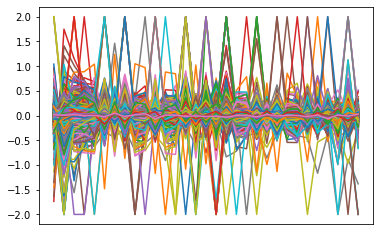
\includegraphics[width=0.4\textwidth]{mo_bic1}}}
    \hspace{.1em}
    \subfigure{}\addtocounter{subfigure}{-2}
    \subfigure{\subfigure[编号b]{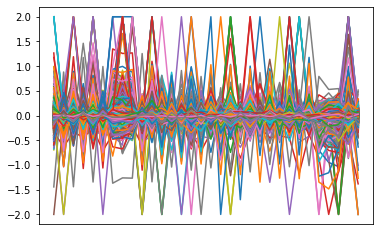
\includegraphics[width=0.4\textwidth]{mo_bic2}}}
    \end{minipage}
    \vspace{0.2em}
    \caption{MOBFO在YC数据集上两个双聚类的基因分布情况}
    \label{fig:mobfo_bics}
    \end{figure}

    \subsection{MOBFOB算法的质量评价指标的比较分析}
    图\ref{fig:mobfo_bcll}到图\ref{fig:mobfo_rat}分别是MOBFO算法在各数据集上,每次趋化操作后种群最小适应值的变化曲线。从图中可以看出,尽管在GV和CV指标上会出现明显的起伏,但是总体的趋势还是下降的。需要额外提示的是,纵坐标为GV和CV的负数,越低则容量越大。而MSR一直在稳步下降,这是因为在进行趋化操作时,对于MSR的权重是最大的,所以算法会在两个解互不支配时,牺牲一部分容量来换取MSR的下降,这也解释了GV和CV的起伏。同时,注意到算法在后期会有一定程度的发散,这是因为Levy飞行以及细菌觅食算法是具有随机性的,这有助于提高种群的多样性和跳出局部最优。

    \begin{figure}[htbp]
    \setlength{\subfigcapskip}{-1bp}
    \centering
    \begin{minipage}{.9\textwidth}
    \centering
    \subfigure{}\addtocounter{subfigure}{-2}
    \subfigure{\subfigure[MSR]{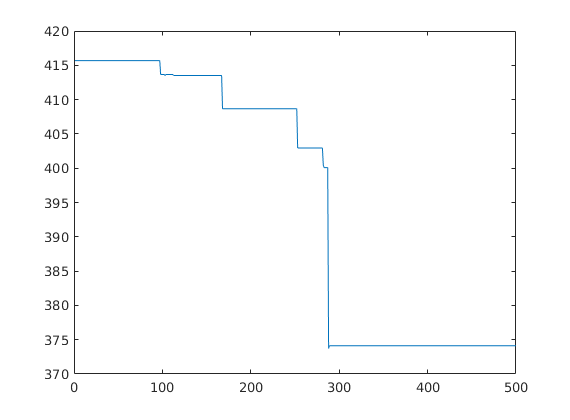
\includegraphics[width=0.3\textwidth]{mo_bcll_msr}}}
    \hspace{.1em}
    \subfigure{}\addtocounter{subfigure}{-2}
    \subfigure{\subfigure[GV]{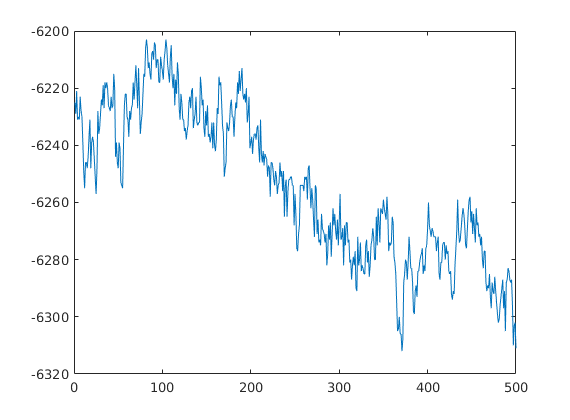
\includegraphics[width=0.3\textwidth]{mo_bcll_gv}}}
    \hspace{.1em}
    \subfigure{}\addtocounter{subfigure}{-2}
    \subfigure{\subfigure[CV]{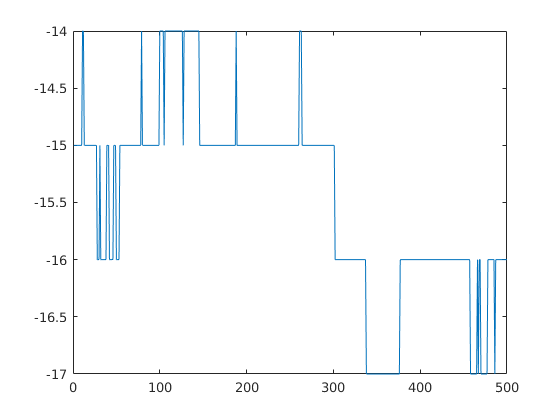
\includegraphics[width=0.3\textwidth]{mo_bcll_cv}}}
    \end{minipage}
    \vspace{0.2em}
    \caption{MOBFO在BCLL数据集上适应值变化曲线}
    \label{fig:mobfo_bcll}
    \end{figure}

    \begin{figure}[htbp]
    \setlength{\subfigcapskip}{-1bp}
    \centering
    \begin{minipage}{.9\textwidth}
    \centering
    \subfigure{}\addtocounter{subfigure}{-2}
    \subfigure{\subfigure[MSR]{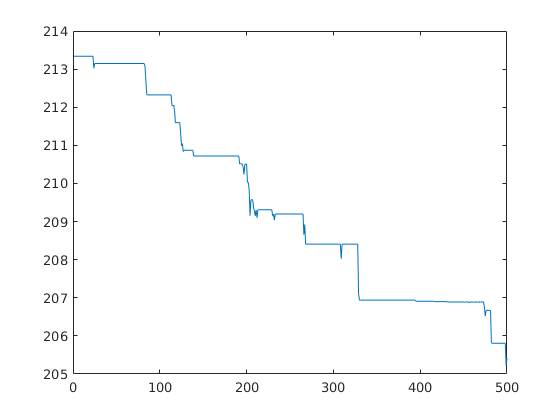
\includegraphics[width=0.3\textwidth]{mo_pbc_msr}}}
    \hspace{.2em}
    \subfigure{}\addtocounter{subfigure}{-2}
    \subfigure{\subfigure[GV]{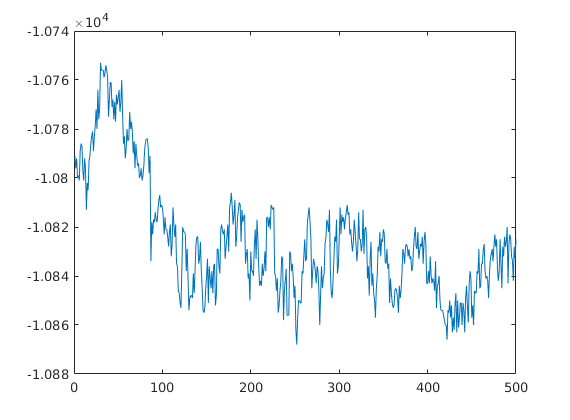
\includegraphics[width=0.3\textwidth]{mo_pbc_gv}}}
    \hspace{.2em}
    \subfigure{}\addtocounter{subfigure}{-2}
    \subfigure{\subfigure[CV]{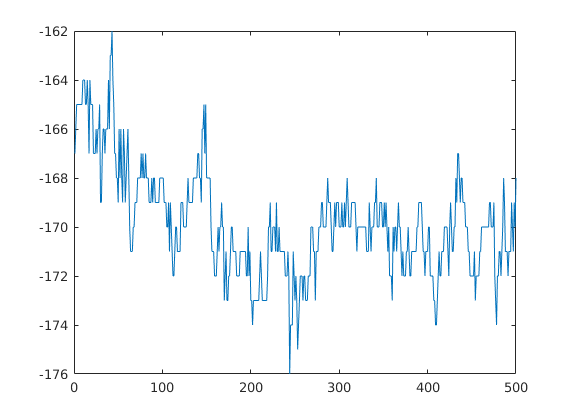
\includegraphics[width=0.3\textwidth]{mo_pbc_cv}}}
    \end{minipage}
    \vspace{0.2em}
    \caption{MOBFO在PBC数据集上适应值变化曲线}
    \label{fig:mobfo_pbc}
    \end{figure}

    \begin{figure}[htbp]
    \setlength{\subfigcapskip}{-1bp}
    \centering
    \begin{minipage}{.9\textwidth}
    \centering
    \subfigure{}\addtocounter{subfigure}{-2}
    \subfigure{\subfigure[MSR]{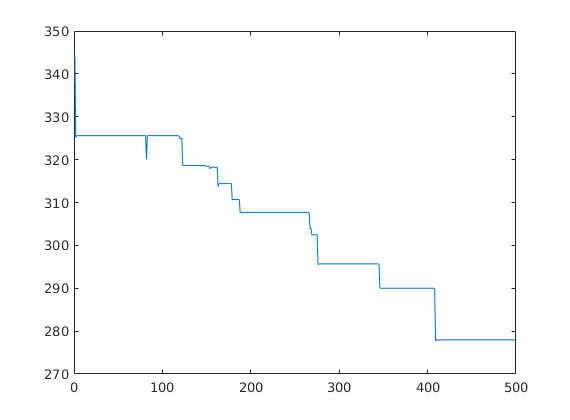
\includegraphics[width=0.3\textwidth]{mo_yc_msr}}}
    \hspace{.2em}
    \subfigure{}\addtocounter{subfigure}{-2}
    \subfigure{\subfigure[GV]{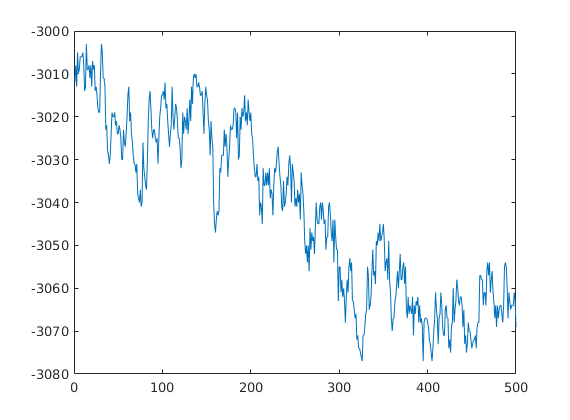
\includegraphics[width=0.3\textwidth]{mo_yc_gv}}}
    \hspace{.2em}
    \subfigure{}\addtocounter{subfigure}{-2}
    \subfigure{\subfigure[CV]{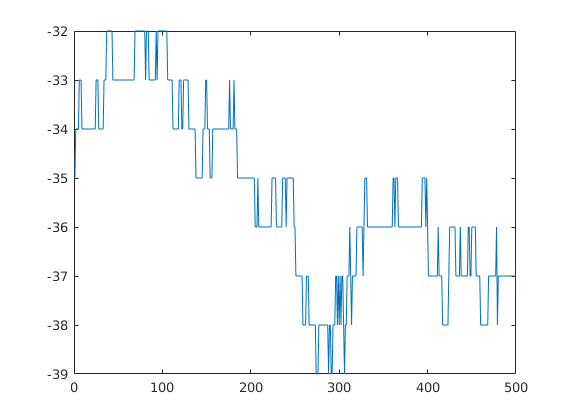
\includegraphics[width=0.3\textwidth]{mo_yc_cv}}}
    \end{minipage}
    \vspace{0.2em}
    \caption{MOBFO在Yeast Cell数据集上适应值变化曲线}
    \label{fig:mobfo_yc}
    \end{figure}

    \begin{figure}[htbp]
    \setlength{\subfigcapskip}{-1bp}
    \centering
    \begin{minipage}{.9\textwidth}
    \centering
    \subfigure{}\addtocounter{subfigure}{-2}
    \subfigure{\subfigure[MSR]{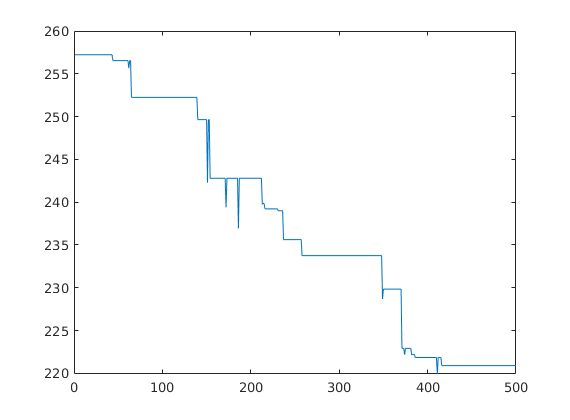
\includegraphics[width=0.3\textwidth]{mo_rat_msr}}}
    \hspace{.2em}
    \subfigure{}\addtocounter{subfigure}{-2}
    \subfigure{\subfigure[GV]{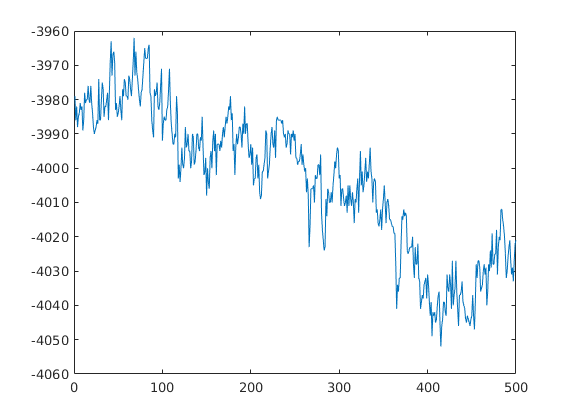
\includegraphics[width=0.3\textwidth]{mo_rat_gv}}}
    \hspace{.2em}
    \subfigure{}\addtocounter{subfigure}{-2}
    \subfigure{\subfigure[CV]{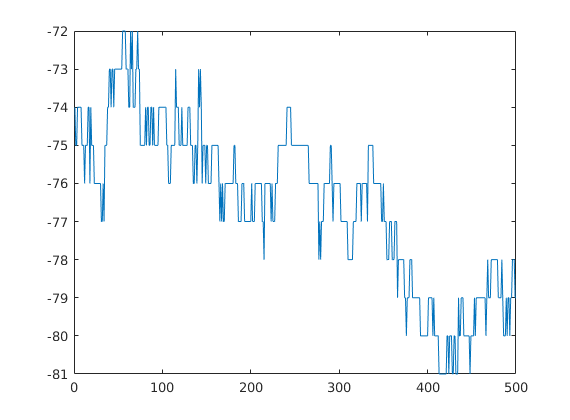
\includegraphics[width=0.3\textwidth]{mo_rat_cv}}}
    \end{minipage}
    \vspace{0.2em}
    \caption{MOBFO在RatStrain数据集上适应值变化曲线}
    \label{fig:mobfo_rat}
    \end{figure}
    从适应值的迭代变化曲线可以看出,算法能够在可行域上找到MSR较低但容量高的双聚类,为了更准确的表示双聚类算法的性能,表\ref{tab:mobfo}为MOBFOB算法在各数据集上的各质量指标的平均值和标准差。跟\ref{sec:csfa_exper}节中的实验数据相比,MOBFOB并没有很突出的表现,这也不足为奇。但是,MOBFOB由于外部集保存了多个帕雷托解,所以在执行效率上有着比单目标优化算法足够多的优势。
    
    \begin{table}[htbp]
        \caption{MOBFOB在各数据集上的质量指标的平均值和标准差}\label{tab:mobfo}
        \vspace{0.5em}\centering\wuhao
        \begin{tabular}{ccccc}
        \toprule[1.5pt]
         & BCLL & Yeast Cell & RatStrain & PBC\\
        \midrule[1pt]
        MSR   &$408.103\pm 54.16$& $344.99\pm 18.57$& $253.95\pm 13.15$& $215.49\pm 4.27$ \\
        GV   &$6154.86\pm 65.08$& $2954.80\pm 31.75$& $3912.67\pm 38.76$ & $10651.02\pm 80.24$\\
        CV   &$9.41\pm 2.82$& $27.05\pm 4.38$& $63.55\pm 7.86$& $156.78\pm 10.98$ \\
        RI   &$-0.00093\pm 0.00309$& $0.00053\pm 0.00432$& $0.00101\pm 0.00559$& $0.00071\pm 0.00143$ \\
        Var   &$468.17\pm 44.06$& $360.074\pm 17.46$& $263.75\pm 13.07$& $221.19\pm 4.42$ \\
        HV   &$0.98\pm 0.004$& $0.99\pm 0.001$& $0.97\pm 0.004$&  $0.98\pm 0.001$\\
        \bottomrule[1.5pt]
        \end{tabular}
    \end{table}

    \subsection{MOBFOB算法的生物评价指标的比较分析}
    为了验证MOBFOB算法能够找到具有生物意义的双聚类,本文对得到的双聚类进行了详细的GO分析,生物验证指标的平均值和标准差如表\ref{tab:mobfo_go}所示。图\ref{fig:go_bcll}给出了MOBFOB在BCLL数据集上的某个双聚类(编号1)GO分析后部分较为显著的GO项,其中包括了15个生物过程(Biological Process),10个细胞组成(Cellualr Component),15个分子功能(Molecular Function)。该双聚类由4529个基因和7个样本组成。由图\ref{fig:go_bcll}可知,该双聚类对于生物过程的富集程度要高于其他两种,其次是细胞组成,分子功能最低,而且所富集的GO项和相关的基因个数都表明了其具有一定的生物意义。  

    \begin{table}[htbp]
        \caption{MOBFOB在各数据集上的生物验证指标的平均值和标准差}\label{tab:mobfo_go}
        \vspace{0.5em}\centering\wuhao
        \begin{tabular}{ccccc}
        \toprule[1.5pt]
         & BCLL & Yeast Cell & RatStrain & PBC\\
        \midrule[1pt]
        WEScore   &$231.37\pm 13.98$& $46.15\pm 8.38$& $137.07\pm 48.68$& $138.07\pm 11.49$ \\
        meanPValue   &$4.89\pm 0.13$& $4.67\pm 0.40$& $4.87\pm 1.18$ & $4.24\pm 0.12$\\
        rateGeneTerm   &$1.71\pm 0.06$& $1.57\pm 0.18$& $0.16\pm 0.05$& $3.32\pm 0.22$ \\
        \bottomrule[1.5pt]
        \end{tabular}
    \end{table}

    \begin{figure}[htbp]
        \centering
        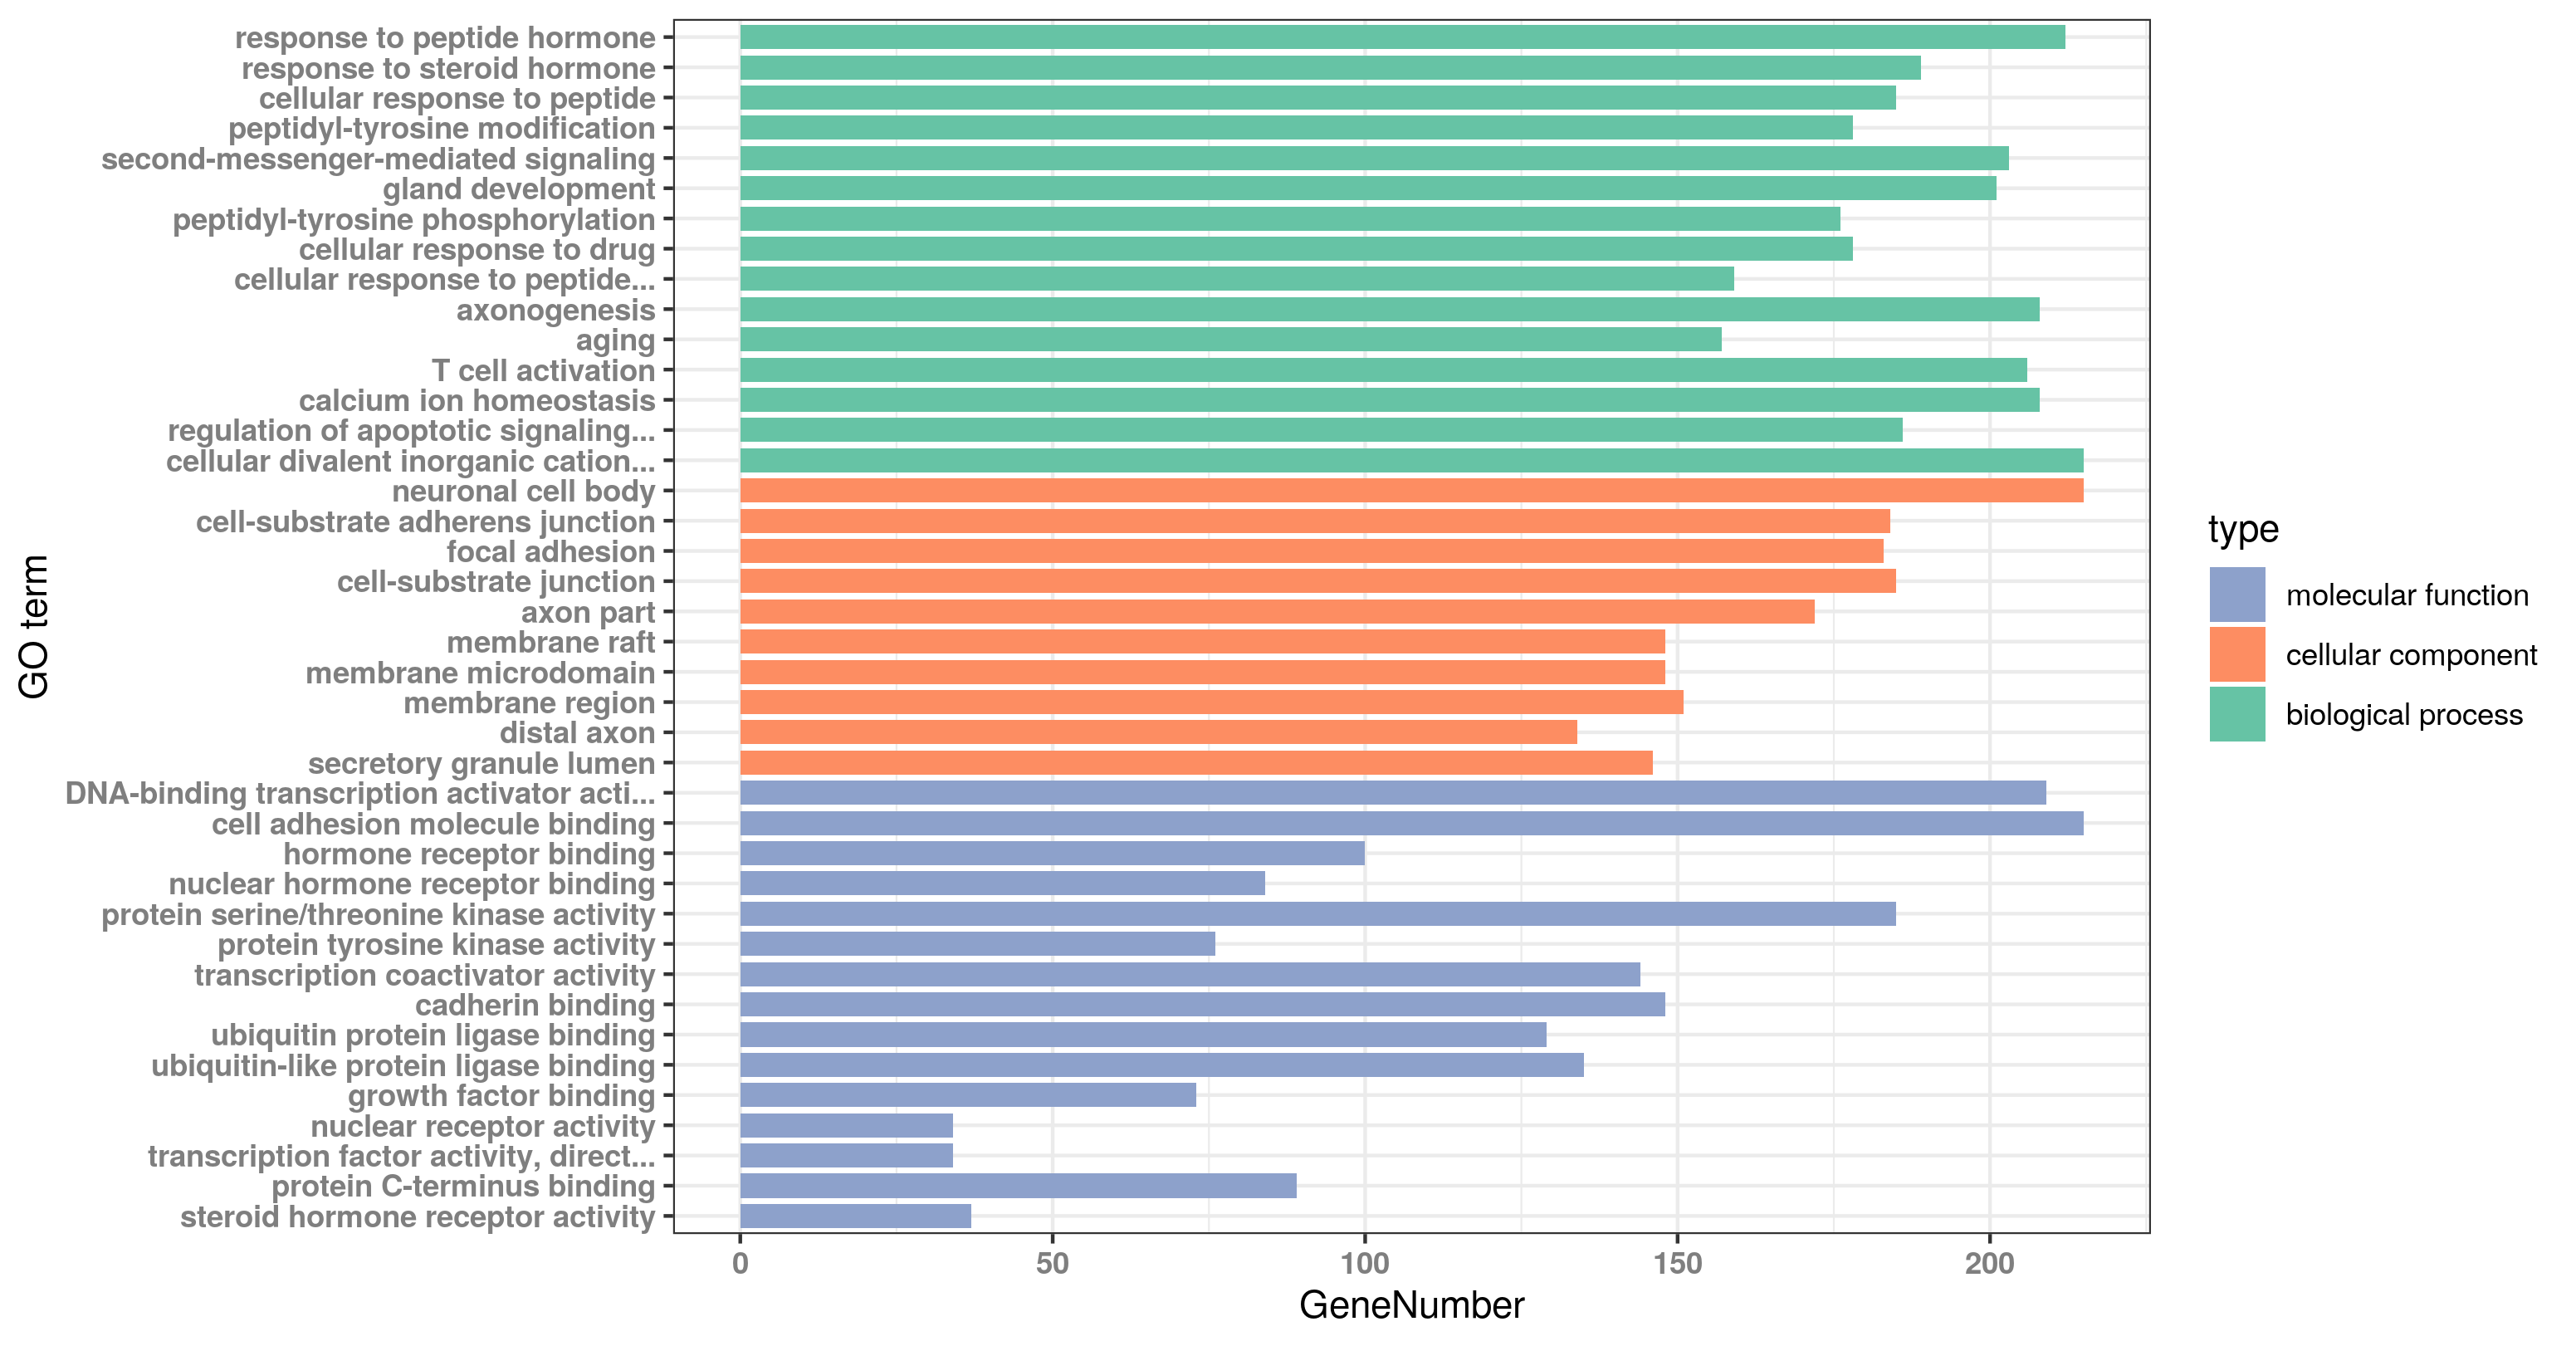
\includegraphics[width = 1\textwidth]{mo_go_bcll_1}
        \caption{MOBFOB算法得到的双聚类(编号1)主要的GO项}
        \label{fig:go_bcll}
    \end{figure}
    表\ref{tab:go_term}为双聚类(编号1)相关GO项的详细信息。例如,表中第二行对应的ID为GO:0048545,该GO项代表的是生物过程中对类固醇激素的反应,4529个基因中有189个与该GO项相关,从BCLL数据集上随机选择4529个基因至少包含这189个基因的概率是4.52E-23。该双聚类中有184个基因参与到了GO:0005924中,该项的描述为细胞组成中的细胞-基质粘附连接,其调整后的P值为2.68E-20。这说明了该双聚类的基因集合中存在功能紧密相关的子集合,形成了一种明显的基因表达模式。

    \begin{table}[htbp]
        \caption{双聚类(编号1)相关GO项的详细信息}\label{tab:go_term}
        \vspace{0.5em}\centering\wuhao
        \begin{tabular}{cccccc}
        \toprule[1.5pt]
        GOID & GO类别 &调整P值 &  基因个数 & GO描述\\
        \midrule[1pt]
        GO:0043434 &生物过程 &3.74E-25& 212& response to peptide hormone \\
        GO:0048545 &生物过程 &4.52E-23& 189& response to steroid hormone \\
        GO:0019932 &生物过程 &3.53E-21& 203& second-messenger-mediated signaling \\
        GO:0043025 &细胞组成 &1.37E-20& 215& neuronal cell body \\
        GO:0005924 &细胞组成 &2.68E-20& 184& cell-substrate adherens junction \\
        GO:0004674 &分子功能 &2.23E-12& 185& protein serine/threonine kinase activity \\
        GO:0050839 &分子功能 &1.77E-15& 215& cell adhesion molecule binding \\
        \bottomrule[1.5pt]
        \end{tabular}
    \end{table}

\section{本章小结}
本章为了解决单目标优化的效率问题,将细菌觅食算法的多目标版本用于双聚类分析。首先简要介绍了多目标优化中的相关概念,然后结合多目标优化和细菌觅食算法的特点,提出了MOBFOB算法。实验先是通过双聚类的基因分布情况直观地观察双聚类的变化一致性,接着又从质量验证指标和生物验证指标证明了算法的有效性,即能够在迭代中优化多个目标,并最终得到有显著生物意义的双聚类,达到预期目标。